\chapter{Scientific Data Analysis with Excel}
\thispagestyle{fancy}
\fancyhead[RE,LO]{Technical Document \thechapter}
\label{chap:excel-analysis}
%
Excel (or any spreadsheet program) can help you do calculations quickly and efficiently. 
But Excel is only a software program — it can only be as smart as the instructions that you give to it.
This technical document will walk you through all the basic steps that you will need to use in each experiment to properly analyze your data.
Each version of Excel (as with the other Microsoft Office programs) varies slightly, but familiarity with one version should help you intuitively guess/explore the other versions. 
Some of you may feel that you are already familiar with Excel; please READ this Technical document anyway! 
It contains specific scientific norms that you need to learn.

\section*{Entering Data:}
%\includegraphics[width=\linewidth]{exAn1}
%In a blank/new Excel document:
%\par 
To enter information in a cell, click on the cell (e.g., cell A1—column A, row 1) and type the information. 
When you are finished, press `Enter.' 
You will see the information in the cell. 
To edit the information, click on the cell and type (erases previous entry) or click on the cell and then click on the formula bar to edit (the formula bar is above all the cells but below all the icons for text manipulation (bold, italicize, center in cell, etc.).
\par 
When you are entering data into excel, begin by adding a title to each column with the quantity's name and units.
In the cells beneath each column title, enter the data that you have collected by typing the numbers into the cells.
When you have finished entering your data, save the file by pressing `Ctrl' + `S' (name the file and note the saved location for future use) or by selecting the `File' tab, then the `Save as' icon. 
Save regularly to avoid losing work.
Every time you save the file, it overwrites the previous version.
\par 
The number of decimal places displayed in the cell can be controlled by icons in the `Number' menu on the `Home' tab.
Use these icons to give your data uniform appearance.

\section*{Generating Columns of Data Calculated from a Formula:}
To generate information from a formula (i.e., to mathematically manipulate cells), click on a cell and begin with =. 
All Excel entries for which you expect a numerical result/output MUST begin with an equals sign, =. 
The mathematical manipulators are what you would expect: * to multiply, / to divide, + to add, and – to subtract. 
To exponentiate, type \char`\^ \ and the power (e.g., $6^{2}$ is 6\char`\^2). 
Let's say you wished to multiply the entry in cell A1 by 60. 
To do this you would click on the cell where you wish the output to go and then type:

\medskip
\texttt{=60*A1}
\medskip

You can type the input cell, A1, on the keyboard, or you can use the mouse to click on cell A1 while typing the formula. 
For more complex mathematical operations, parentheses often become necessary. 
Excel will color-code the parenthesis to help you see where each set opens and closes. 
Be VERY careful with your parentheses!
(Again, Excel is only as smart as the instructions that you give to it!)
\par 
If you wish the same mathematical formula to be applied to every cell in a column (e.g., column F is column A times 60), type the formula into the output cell for the first row. 
Then click on the output cell and move your mouse over the bottom, right corner of the cell. 
Your pointer will change shape and become a plus. 
Click the left mouse button, drag down to the last cell you wish to effect, then release the mouse button (you can also double click the bottom left corner). 
The cells will automatically fill in. 
By clicking on any of these cells, you can see in the formula bar that the formula has been adjusted to reference the correct input cell (i.e., for the row you are currently in). 
The same process can be used to copy a formula across a row into multiple columns. 
If, in a formula, you wish to reference a specific column or cell (that will NOT change when the formula is dragged over a column or row), use the \$ symbol: e.g., \$A1 will always be column A, but the row number can change; and \$A\$1 will always be column A and row 1 — neither can change. See the example below in figure~\ref{fig:exc1}:

\begin{figure}[ht]
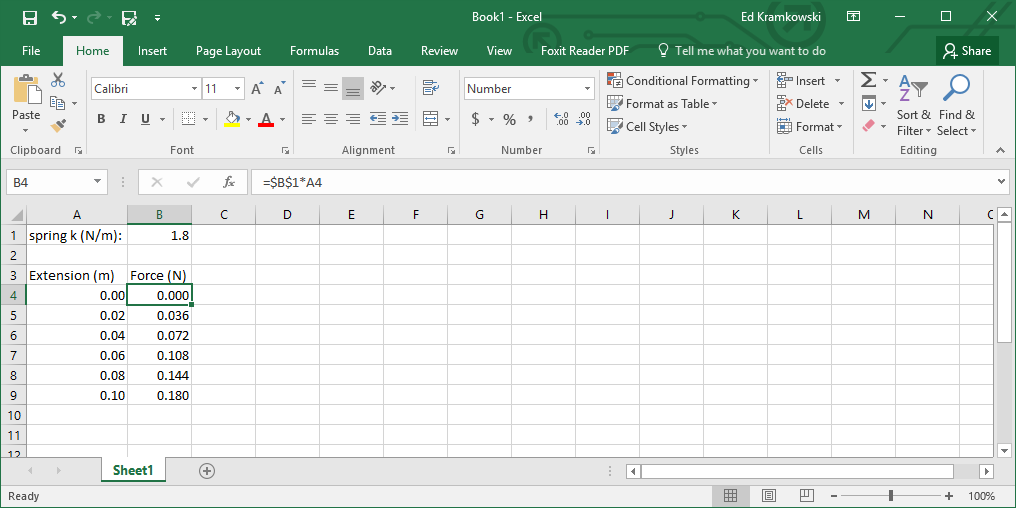
\includegraphics[scale=0.5]{excel1.png}
\centering
\caption{An example of using the \$ symbol to use a constant in a calculation. The force of a spring is calculated using $F=k * x$, where k is the spring constant and x is the extension of the springs length.}
\label{fig:exc1}
\end{figure}

Another example is shown in figure~\ref{fig:exc2} on page~\pageref{fig:exc2}.

\begin{figure}[ht]
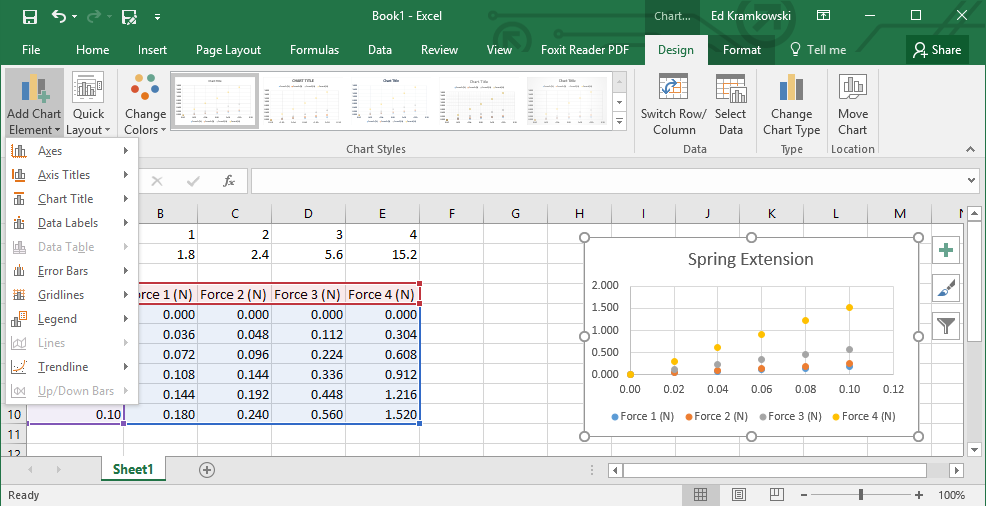
\includegraphics[scale=0.5]{excel4.png}
\centering
\caption{To add other elements to your chart (e.g. axis titles), choose ``Add Chart Elements'' from the ``Design'' menu.}
\label{fig:exc4}
\end{figure}

\section*{Generating Graphs:}
When creating a graph/plot, Excel will usually plot the first column on the independent/ horizontal axis and the second column on the dependent/vertical axis. 
You should always check that the correct data has appeared on the correct axis. 
If the data has been entered with the columns in reverse order, this can be fixed after the plot is created.
\par
To generate a graph/plot, use the mouse to highlight the data that you wish to graph (if the data is adjacent, just highlight the entire chunk; if the columns are not adjacent, highlight each column separately while holding the `Ctrl' key). 
Once the data is highlighted, click on the `Insert' tab and then the `Scatter' icon (on the `Charts' menu - other types of charts may be appropriate for different data types, but the Scatter plot is the most commonly used). 
From the sub-types of scatter plot available, choose the one that has data points but no lines. 
A graph will appear — but you are NOT finished yet!
\par
The design of the graph can be adjusted using the `Chart Layout' menu (see figure~\ref{fig:exc4}) - you will want to be able to label the individual axes with the quantity graphed and its units and you will want to be able to title the graph. 
When the graph has been titled (for the `vs.' format, it is always `Dependent' vs. `Independent') and the axes have been properly labeled, you can choose to keep or delete the Legend (not needed if only one data set is plotted, absolutely necessary for multiple data sets). 
The location of the chart can be changed by: left-clicking on the chart (the upper right corner works well), then right clicking and choosing `Move Chart' from the menu. 
It is often best to make the chart a `New Sheet' (so that it doesn't block your view of the data) - give it an appropriate title and click `Okay.' 
You chart will become its own sheet - and your data will disappear! 
But the data is not gone - to find it, use the tabs on the bottom of the Excel window (`Sheet 1' is usually the data; now might be a good time to rename it `Data': right click, select `Rename' and name it).
\par 
Before you finish, check that the correct data has been plotted on the correct axis and that the axis labels match the quantities plotted (see figures~\ref{fig:exc5} and \ref{fig:exc6}). 
If the original columns were in reverse order, this can be adjusted by left-clicking on a data point (to select the data), and then right-clicking and choosing `Select Data.' 
Click on the Legend Entry you wish to adjust, and then click `Edit.' 
Highlight the appropriate Series X and Series Y data and then click `Okay.'

\section*{Making Good Graphs}
One thing you should focus on in this class is developing good graph-construction habits.
Presenting data in a graph that is both accurate and easy to follow is an important skill to have in any scientific discipline. \\
When formatting your graphs:
\begin{itemize}
\itemsep-0.3em
\item Give your graph a descriptive title.
\item Make sure that all axes are labeled at a legible font size; do not forget to include units.
\item If you are graphing discrete data points (as will be the case most often), use only the basic scatter plot.
\item If your graph contains multiple independent data sets, be sure to include a legend.
\item Include a caption giving a short description of your graph. Make sure to note any important features.
\end{itemize}
\begin{figure}[ht]
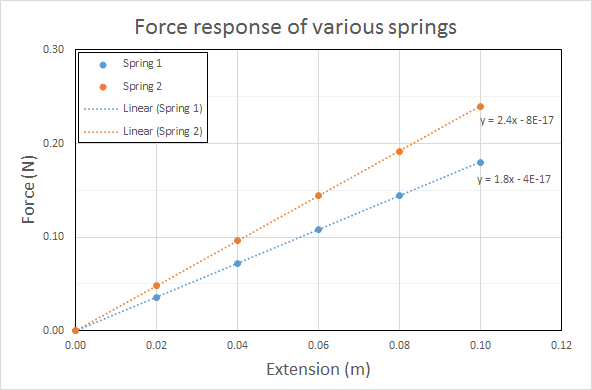
\includegraphics[scale=0.7]{excel3.png}
\centering
\caption{An example of properly graphed data. The data was plotted using a scatter plot. Trendlines (and their equations) were then added.}
\label{fig:exc3}
\end{figure}

\section*{Adding a Best Fit (``Trendline'') to a Graph:}
To add a line of fit (called a ``Trendline'' in Excel) to a graph:
\begin{itemize}
\itemsep-0.3em
\item Left-click on a data point to select the data series that you want to add a trendline for.
\item Right-click on the same data point and choose `Add Trendline.' 
\item The trendline formatting options should open on the right side of the program. Choose the appropriate Trend/Regression type, and tick the boxes for `Display Equation on chart' and `Display R-squared value on chart.' 
\item As a general rule, do not `Set Intercept' to a specific number (i.e., do not force the origin to be part of the trendline). 
\end{itemize}
Do you know what the R-squared value really means? 
If not, you should look it up! 
Look at the equation for the trendline and think about it. 
What does the slope mean? 
What does the y-intercept mean? What does this R-squared value mean?

\section*{Adding Error Bars to the Data Points on a Graph:}
Error bars represent the uncertainty of the measurement of the data. 
Do you have uncertainty? 
Do you have uncertainty in both quantities (horizontal and vertical)? 
Is the uncertainty the same for all data points, or does it change with the value of the quantity plotted? 
Wherever you have uncertainty, you must have error bars! 
Once you have determined the amount of uncertainty, you can add error bars by following these steps:
\begin{itemize}
\itemsep-0.3em
\item In the Chart Tool's `Design' tab, click `Add Chart Elements > Error Bars > More Error Bars Options...'. 
\item If you have multiple sets of data in the same chart, select the data series that you are adding error bars too.
\item The format window should open on the right. You can adjust the length of the error bars by selecting one of the options under `Error Amount'.
\item Apply the error bars according to the decisions that you have made about your uncertainty; a good choice is often `Standard Error', but you may sometimes wish to use errors that you calculated by selecting `Custom' and then selecting the appropriate cells with your errors. 
\item To remove either vertical or horizontal error bars, left-click on the bars, then right-click and choose `Delete'.
\end{itemize}

\section*{Other cool tools:}
As a spreadsheet program, Excel can do a lot of useful statistical analysis and mathematical manipulation. 
Some functions you will find useful include: Sum, Average, and Standard Deviation.
\par 
To \textbf{Sum} elements, click on the cell in which you wish the result to appear, then enter \texttt{=sum}. 
Immediately, Excel will list possible formula options that begin with \texttt{sum}. 
For a simple summation of elements, you would choose the SUM function, which you have already typed, but you should note the other options available. 
Open parentheses following your sum, so that you have now types \texttt{=sum(} and then highlight the cells to be summed. 
Close your parentheses and press `Enter.' 
(It would look like this \texttt{=sum(A1:A5)} for a sum of the cells in rows 1 through 5 of column A.)
\par 
To \textbf{Average} elements, click on the cell in which you wish the result to appear, and then enter \texttt{=average(}. Highlight the cells you wish to average and then close your parentheses and press `Enter.' 
Note that Excel will offer you a list of average functions - the most commonly used option is the AVERAGE function. (It would look like this \texttt{=average(A1:A5)} for the average of the cells in rows 1 through 5 of column A.)
\par 
To perform a \textbf{Standard Deviation} on a set of elements, click on the cell in which you wish the result to appear, and then enter \texttt{=stdev.s(}. 
Highlight the cells you wish to perform a standard deviation upon and then close your parentheses and press `Enter.' 
Note that Excel will offer you a list of standard deviation functions - the most commonly used option is the STDEV.S function. 
(It would look like this \texttt{=stdev.s(A1:A5)} for the standard deviation of the cells in rows 1 through 5 of column A.)
\par 
To perform any of these functions on disconnected sets of cells (e.g., cells in rows 1 through 13 and then 15 through 17), open your parentheses, highlight the first contiguous group, enter a comma, then highlight the next contiguous group, enter a comma, and so forth, continuing to the last group of numbers and ending with a closing parenthesis and the `Enter' key. 
(As an example, \texttt{=average(A1:A13,A15:A17)}.)
\par 
Excel has many other functions available, including trigonometric and logarithmic functions. 
Investigate what is available by clicking on the `Formulas' tab and looking through the `Function Library,' especially the `Math \& Trig' and `More Functions' menus.

\section*{Other Examples}

\begin{figure}[ht]
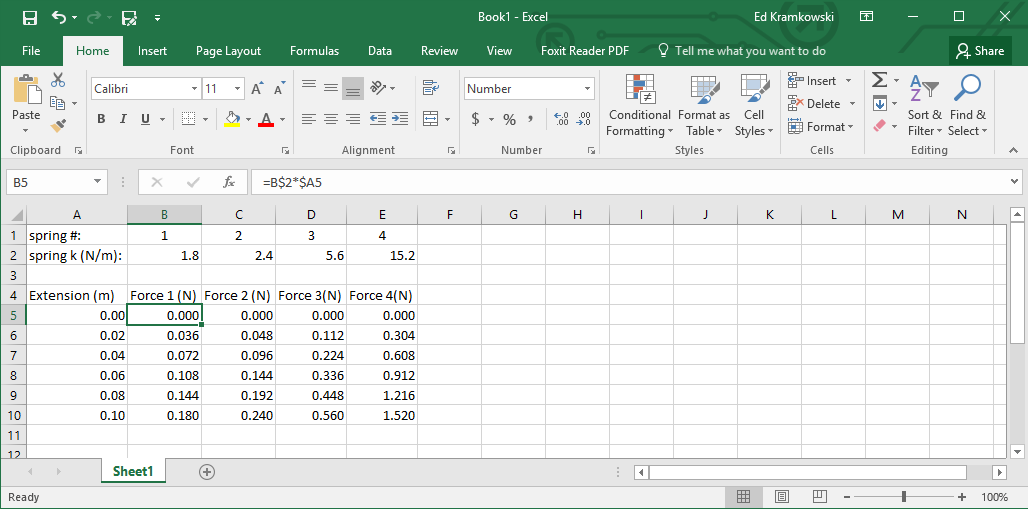
\includegraphics[width=0.8\textwidth]{excel2.png}
\centering
\caption{Another example of using the \$ symbol to use a constant in a calculation. By typing the formula \texttt{=B\$2*\$A5} into cell B5, you can allow the constant to change along a specified axis, while continuing to multiply by the numbers in the `Extension' column.}
\label{fig:exc2}
\end{figure}

\begin{figure}[ht]
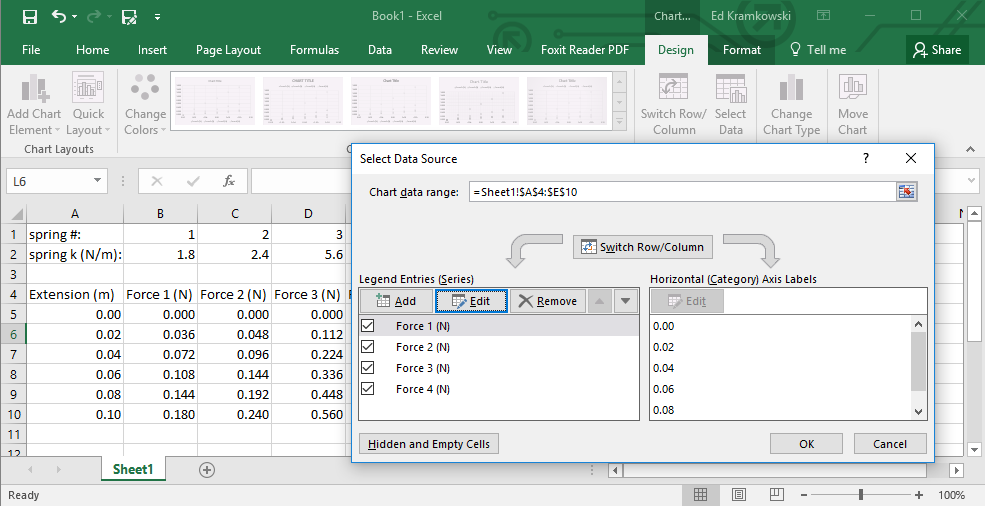
\includegraphics[width=0.8\textwidth]{excel5.png}
\centering
\caption{To edit or add sets of data to a graph, choose ``Select Data'' from the ``Design'' menu.}
\label{fig:exc5}
\end{figure}

\begin{figure}[ht]
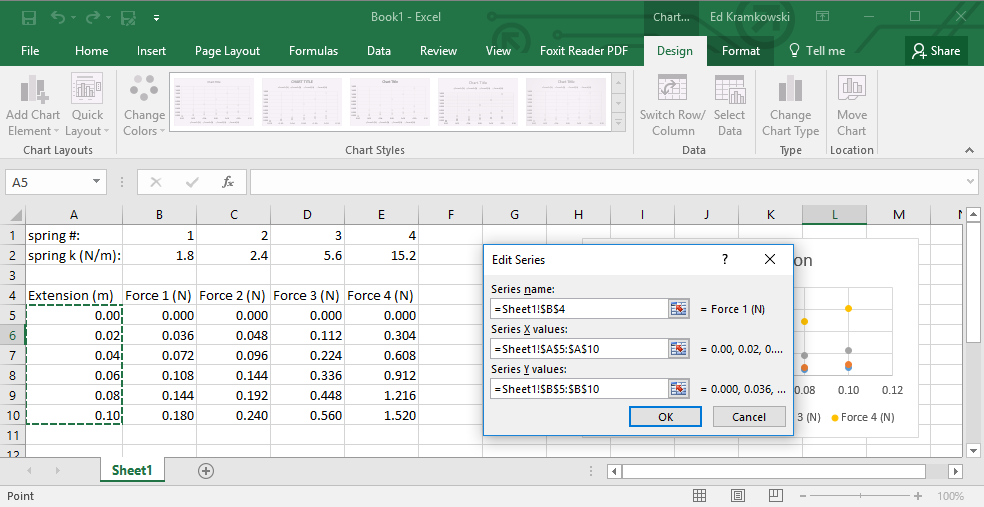
\includegraphics[width=0.8\textwidth]{excel6.png}
\centering
\caption{After selecting ``Edit'' in the ``Select Data Source'' menu, you can check if the values are being graphed on the proper axes, and edit the size of the data series if necessary.}
\label{fig:exc6}
\end{figure}